\chapter{Analyse - État de l'art}
\label{ch:analysis}
Ce chapitre va s'intéresser aux différentes propositions d'implémentations de système de messagerie sécurisée afin de voir où en est l'état de l'art. Pour les systèmes les plus connus tels que PGP et S/MIME sont analysés mais aussi les implémentations de ces protocoles dans des clients mails tel que Protonmail ou Tutanota. L'analyse s'élargit aussi à des protocoles plus orientés vers la messagerie instantanée comme Signal.

\section{Système de messagerie}
Dans un système de messagerie les besoins principaux sont surtout de pouvoir consulter sa boîte mail à tout moment avec les anciens et nouveaux emails reçus. De plus, il est préférable de pouvoir envoyer des emails aussi. Ces envois peuvent avoir plusieurs propriétés et fonctionnalités. On pourrait envoyer un email à de multiples destinataires et même sans que les uns et les autres sachent exactement à qui est envoyé l'email exactement (copies cachées). Un client mail permet aussi d'envoyer des pièces jointes, celles-ci seront encodées au sein du message et envoyées avec. Un email a aussi un état pour savoir s'il a déjà été lu ou non. Parmi l'utilisation simple d'un système de messagerie il y aussi le fait que l'on veut pouvoir voir ses emails de n'importe quel appareil à n'importe quel moment. Des possibilités de suivis sont généralement possible, afin de savoir si le destinataire a reçu / lu l'email. Il est aussi généralement possible de donner un importance à certains emails.

\subsection{Détails techniques}
Afin d'établir les futures notations utilisées ci-après et montrer le fonctionnement global d'un système de messagerie électronique la Figure \ref{fig:mailGlobal} sera la base de l'explication. Dans cette Figure l'on peut voir que 3 protocoles différents sont utilisés pour la gestion des emails ; SMTP, IMAP et POP3. Ces 3 protocoles sont utilisés par différents acteurs, le MUA (Mail User Agent), le MTA (Mail Transfer Agent) et le MDA (Mail Delivery Agent).

Le MUA est en fait un client mail qui va s'occuper d'envoyer des emails ou de les recevoir (rechercher sur le MDA). 
 
 Les MTAs sont les serveurs de messagerie responsables du bon acheminement des emails. Ainsi les 3 protocoles énoncés plus hauts sont soit pour l'envoi et la transmission (SMTP) soit pour la récupération des messages (IMAP et POP3). 
 
 Lors de l'envoi, un MUA va simplement renseigner les destinataires du message ainsi que sa source, son sujet et son message puis le serveur va transmettre ces informations au MTA du domaine de destination qui s'occupera de le transmettre au MDA (souvent les 2 à la fois), celui-ci stocke les emails en attendant qu'un MUA fasse une demande via POP3 ou IMAP. IMAP est souvent préféré car les emails restent ainsi sur le serveur de messagerie et est donc consultable depuis un autre appareil utilisant aussi IMAP. POP3 va plutôt télécharger les emails et les enlever du serveur, ils ne seront donc plus disponibles par le biais d'un autre appareil.
 
 Les MTAs sont des serveurs de transmission de données, transmises en clair jusqu'à l'introduction d'ESMTP et de la directive STARTTLS, permettant un niveau basique de sécurité entre 2 MTAS pour le transfert d'emails. Cependant, si un MTAs est mal configuré et ne permet pas cette directive, l'email transitera en clair. C'est dans ce contexte là ainsi que celui du stockage des emails en clair par le MDA que des solutions de chiffrement d'email en E2E (End to End - Chiffrement de bout-en-bout) ont vu le jour.
 
\begin{figure}[h!]
	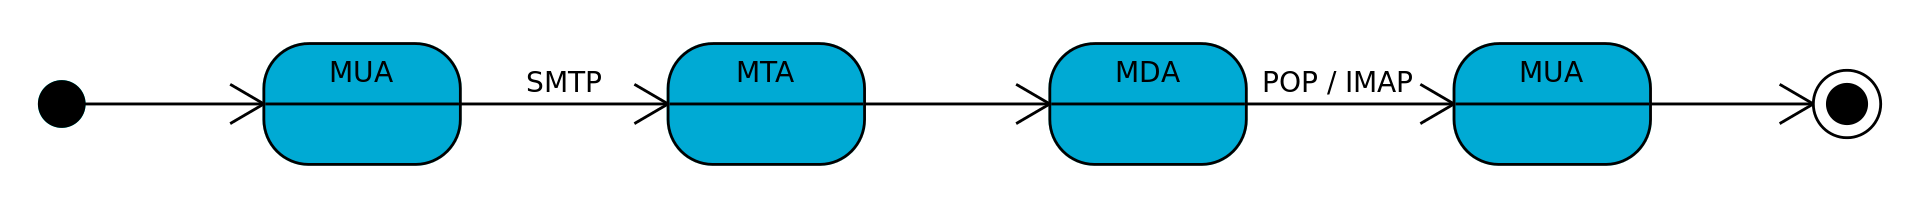
\includegraphics[width=14cm]{images/Etapes_envoi_email.png}
	\centering
	\caption{Le fonctionnement d'un système de messagerie~\cite{mailGlobal}}
	\label{fig:mailGlobal}
\end{figure}

\section{Protocoles existants}
Dans cette section une analyse des différents protocoles existants pour sécuriser la messagerie électronique est proposée. Puis une recherche sur leur implémentation au sein de certains clients emails est faite. De plus, une présentation d'un protocole de messagerie instantanée fortement sécurisé est faite afin de voir s'il est possible d'implémenter cela dans un système d'emails.

\subsection{PGP}

\paragraph*{Fonctionnement.}
PGP (Pretty Good Privacy ou Assez bon niveau de confidentialité) est un moyen de chiffrer des données (emails, fichiers, …). C’est une méthode de chiffrement hybride (utilise le chiffrement symétrique et asymétrique) qui fonctionne comme montré sur la Figure \ref{fig:PGP_101}. Comme on peut le voir, on tire une clé symétrique aléatoirement qui permettra de chiffrer notre email avec un chiffrement symétrique comme AES. Ensuite, on va chiffrer cette clé symétrique à l'aide d'un chiffrement asymétrique, en utilisant la clé publique du destinataire.

\begin{figure}[h!]
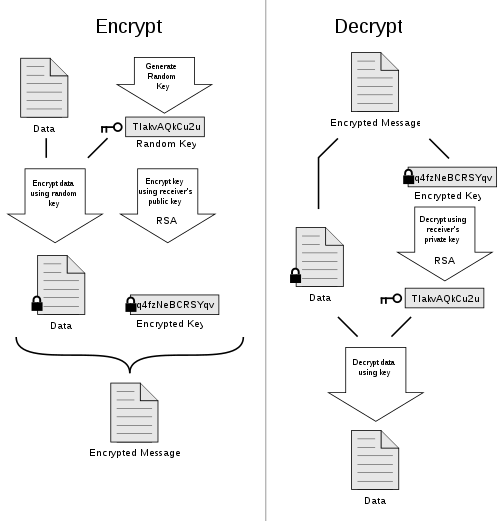
\includegraphics[width=10cm]{images/PGP_101.png}
\centering
\caption{Le fonctionnement global de PGP~\cite{pgpGlobal}}
\label{fig:PGP_101}
\end{figure}

Ce fonctionnement hybride est expliqué par la lenteur d’un chiffrement asymétrique sur un certain nombre de données. Ainsi en chiffrant uniquement la clé symétrique qui a servi à chiffrer le message, le déchiffrement est bien plus rapidement effectué. Typiquement, avec un chiffrement symétrique tel qu’AES ayant des instructions dédiées dans certains processeurs. Contrairement à des chiffrements asymétriques qui sont plus contraignants. Mais il est nécessaire de passer par cette phase asymétrique, on a en effet besoin d'un secret partagé dès le début de la communication si cette méthode n'est pas utilisée.

Pour ce qui est des primitives cryptographiques proposées dans la RFC4880~\cite{RFC4880}, elle sont listées ci-après dans la table \ref{table:refPGPAlgos}.

\begin{table}[h!]
	\centering
	\begin{tabular}{||c c c c||}
		\hline
		Symetric & Asymetric & Hash & Compression \\ [0.5ex]
		\hline\hline
		IDEA & RSA & MD5 & ZIP \\
		TripleDES & ElGamal & SHA-1 & ZLIB \\
		CAST5 & DSA & RIPE-MD160 & BZip2 \\
		Blowfish & ECDSA & SHA256 & \\
		AES-128 & Diffie-Hellman & SHA384 & \\
		AES-192 & & SHA512 & \\
		AES-256 & & SHA224 & \\
		Twofish-256 & & & \\
		IDEA & & & \\
		\hline
	\end{tabular}
\caption{Table des algorithmes utilisés par PGP}
\label{table:refPGPAlgos}
\end{table}

Attention MD5 a été annoncé déprécié. Il faut savoir que pour chacune de ces catégories il y a 10 éléments réservés pour des primitives privées/expérimentales.

Lorsqu'un email est chiffré et signé avec PGP, il est d'abord hasher puis ce hash est signé avec la clé privée de l'utilisateur afin de faire une signature digitale. Le message et la signature sera alors chiffrée à l'aide de la clé symétrique.

L'organisation d'un message PGP se fait via des "paquets" d'informations encodés en base64. La RFC4880~\cite{RFC4880} définit bien ces types de paquets, leur fonctionnement et les différents codes associés. Sur le blog de Conrad Irwin\footnote{\url{https://cirw.in/gpg-decoder/}} l'on peut entrer un message PGP et ainsi voir l'organisation d'un message, ou entrer des clés publiques ou une clé privée (déconseillé tout de même). Ainsi, un exemple d'email envoyé à plusieurs destinataires est représenté dans la Figure \ref{fig:PGP_DECODE}. 

\begin{figure}[h!]
	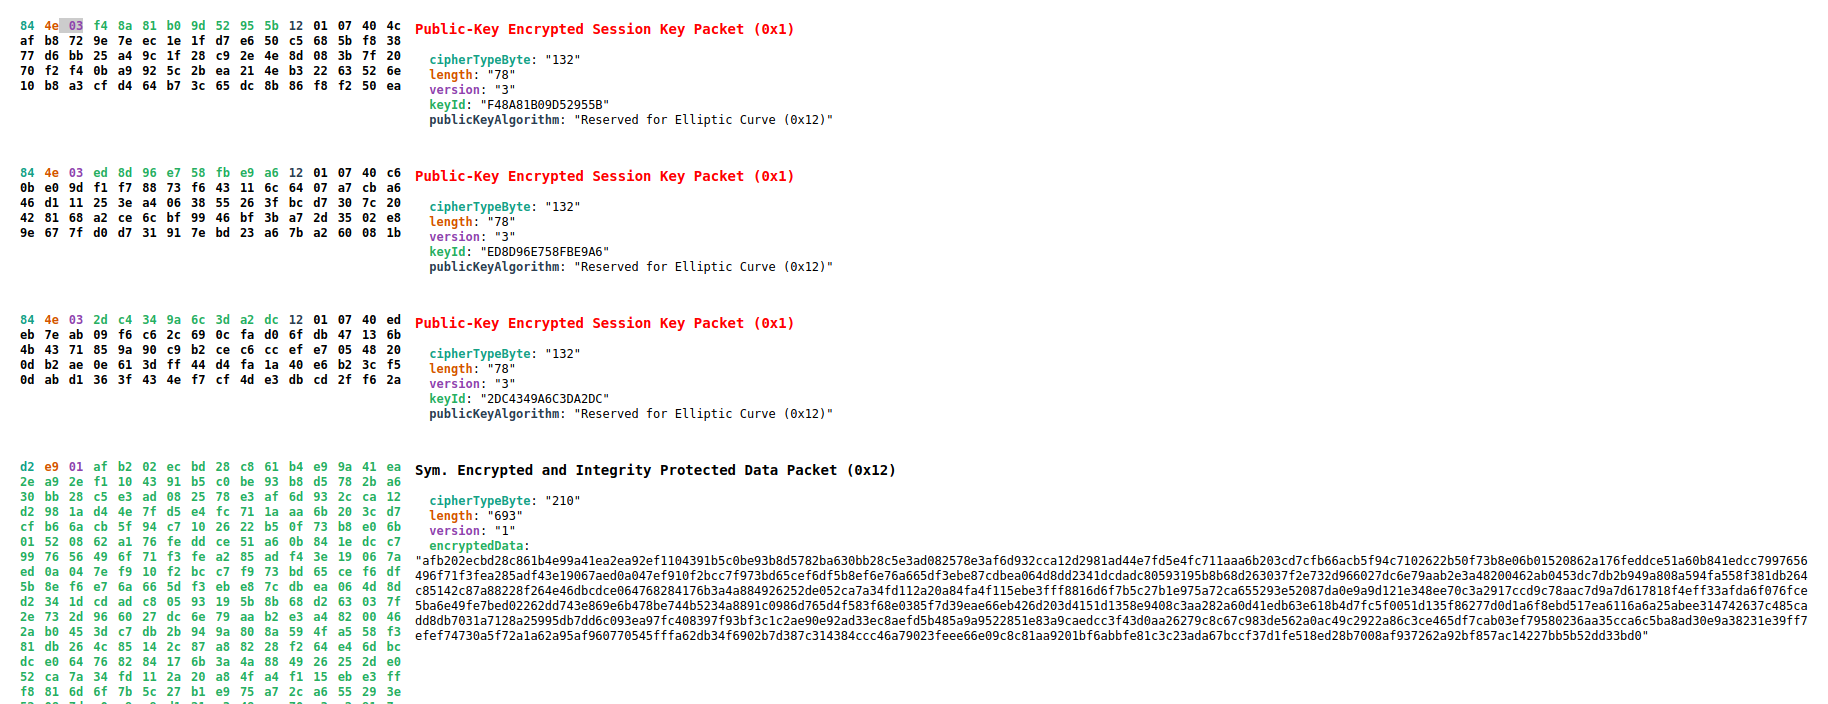
\includegraphics[width=\textwidth]{images/examplePGPDecode.png}
	\centering
	\caption{Exemple décodage d'un message PGP}
	\label{fig:PGP_DECODE}
\end{figure}

Cela démontre comment fonctionnes PGP, en effet le message étant chiffré avec une clé symétrique, le chiffré sera le même pour tout le monde. Mais afin que tous les destinataires puisses avoir la clé symétrique, elle est chiffrée à l'aide des clés publiques des différents destinataires (et de la source, pour pouvoir la déchiffrer à l'avenir et ne pas conserver l'email en clair dans la boite d'envoi). À noter qu'avec l'option de \textit{blind copy} (option permettant d'envoyer à un utilisateur un email sans qu'il sache qu'il a aussi été envoyé à un autre utilisateur), PGP \textit{leak} les receveurs des emails avec leur KeyID qui sera présent dans le message PGP~\cite{BccPrivacy}.

PGP utilise donc un système de clés publiques afin d'envoyer des clés symétriques. Comment obtient-on une clé publique pour envoyer notre message ?

Selon certaines utilisations les clés peuvent être obtenues via un serveur de clés, mais cela implique un parti tier auquel il faut faire confiance, ainsi ce qui peut être fait c'est aussi d'avoir son propre serveur de clés. Mais pour être sûr que tel clé appartienne bien à tel utilisateur, PGP a introduit dès ses débuts un système décentralisé de confiance appelé le "Web of Trust". Ainsi, les utilisateurs signent entre eux leurs certificats d'identité, chacun des utilisateurs aura des clés de confiance et ainsi de suite. Cela permet d'avoir une toile de confiance entres les utilisateurs.

Cependant, ce système est difficile à utiliser, il est nécessaire de faire attention à quelles clés les utilisateurs signent et approuvent. Surtout pour les nouveaux utilisateurs qui ne peuvent faire vérifier leurs clés publiques facilement et ne seront donc pas vérifié. C'est pour cela que des "fêtes" de signature de clés sont organisées afin de se rencontrer personnellement et vérifier que tel utilisateur est bien telle personne. Ces évènements sont d'ailleurs possible grâce aux Fingerprint des clés publiques. Ce sont des chaînes hexadécimales de 20 bytes permettant d'identifier une clé publique plus facilement.

Pour expliquer plus précisément le \textit{Web Of Trust} prenant un exemple : Alice a une clé publique 0xAAAAAAAAAAAA et elle signe la clé de Bob 0xBBBBBBBBBBB car elle le connaît. De la même manière Bob signe la clé publique de Carol 0xCCCCCCCCCCCC. Grâce à cela, Alice peut être sûre que cette clé appartient bien à Carol car il y a un chemin de signature valide entre sa clé publique et celle de Carol. Comme affiché dans la Figure \ref{fig:WOTExample}.

\begin{figure}[h!]
	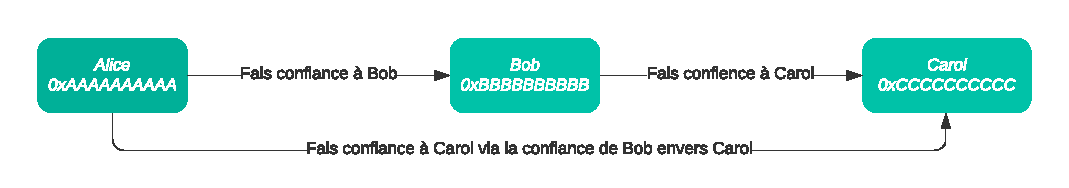
\includegraphics[width=\textwidth]{images/WOTExample.pdf}
	\centering
	\caption{Exemple de la confiance dans le Web Of Trust}
	\label{fig:WOTExample}
\end{figure}

Ces certificats d'identité sont signés à l'aide de SHA-1, cependant il a été prouvé que des attaques sur cet algorithme au niveau des collisions peuvent être faites~\cite{journals/iacr/LeurentP20}. Heureusement, le standard a été modifié dans les nouvelles version de GnuPG pour signer les identités des utilisateurs.

Dans la dernière spécification de PGP des moyens de créer des autorités de certification ont été ajouté afin d'avoir un système décentralisé de \textit{trust signatures}. Ceux-ci ont plusieurs niveaux de confiance définissant s'ils pourront ou non délivrer des signatures. Ceci permet de se baser sur un système qui ressemble à une PKI mais avec une flexibilité sur les CAs (utilisateurs) auxquels on fait confiance ou non.
\paragraph*{Propriétés cryptographiques.}
PGP a surtout été créé pour fournir du \textbf{chiffrement de bout-en-bout} afin de résoudre les problèmes de transmissions en clair entre les MTAs et le stockage des emails en clair dans les MDAs. Ceci même lors d'une récupération d'emails sur un serveur, les emails seraient chiffrés. Ensuite, PGP propose de signer ou non ses emails ce qui amène donc de la \textbf{répudiation} (si non-signé, l'email ne pourra pas être utilisé pour prouver qu'il a été envoyé par telle personne) et \textbf{non-répudiation} (email signé, ainsi on peut prouver que l'envoyeur a bien envoyé l'email).

Le problème qui est souvent reproché à PGP c'est qu'il n'implémente pas de \textbf{Forward Secrecy}. La \textit{Forward Secrecy} permet d'affirmer que si l'on a une brèche à un instant $t$, et qu'un attaquant récupère notre clé privée, il ne pourra pas déchiffrer les anciens messages chiffrés avant l'instant $t$.
\paragraph*{Utilisation.}
Lors des tests, l’utilisation la plus simple possible a été utilisée pour voir si un utilisateur lambda pouvait arriver à mettre en place ce genre de sécurité. Il s’est avéré que cela était assez simple au départ, mais dès lors que l'on veut envoyer un email chiffré à un correspondant cela se complique.

L'installation d'un Add-On sur le logiciel de messagerie (Thunderbird dans ce cas) s’appelant Enigmail, a été nécessaire pour évaluer les cas d'utilisation. Ensuite, Enigmail a généré les clés PGP (de manière totalement automatisée à l'aide GnuPG). Puis l'envoi d'un email se fait simplement via des icônes et des options dans le client de messagerie électronique. Cependant, le fonctionnement est très opaque et on ne sait pas ce qu'Enigmail fait réellement derrière les décors. L’utilisateur doit encore choisir s’il veut chiffrer ses emails ou non. De plus, Enigmail utilise Autocrypt, un système permettant d'envoyer la clé publique directement dans l'email. Cette technologie ne fait pas encore l'unanimité et est donc à utiliser avec précaution.
 
Pour les clés, Enigmail les envoie sur des serveurs de clés par défaut. Il va aussi interroger ces serveurs si une clé publique pour un destinataire est disponible dessus lors du chiffrement d'un message. Ces serveurs sont les suivants : keys.opengpg.org (vks), hkps.pool.sks-keyservers.net (hkps), pgp.mit.edu (hkps). Les protocoles vks (Verifying Keyservers) et hkps (HTTP keyserver protocol over TLS) sont des interfaces avec des serveurs de clés afin d'enregistrer des nouvelles clés ou trouver une clé sur le serveur par différents moyens (email, key-id, fingerprint). Les clés générées ont été générées avec les algorithmes EdDSA 4096bits par défaut, et dans les paramètres avancés il est possible de choisir entre cet algorithme et RSA (algorithme non spécifié).
\subsection{S/MIME}
\label{protocols:SMIME}
\paragraph*{Fonctionnement.}
S/MIME (Secure/Multipurpose Internet Mail Extensions) se base sur un système de PKI (Public Key Infrastructure) pour chiffrer et signer les emails. Dans une telle infrastructure les CAs (Certificate Authorities) garantissent que les certificats décrivent bien l'entité.

MIME est un standard qui étend le format d'email standard afin de pouvoir transmettre des données plus complexes que le format ASCII. En effet, cela permet de transmettre d'autres sets de caractères et la possibilité de transmettre des fichiers joints audio, vidéo, images, programmes aux emails. MIME permet de séparer le message en partie, c'est d'ailleurs là dessus que l'attaque EFAIL (c.f. Section \ref{attacks:EFAIL}) s'appuie. Ces parties ont différent format de données et le message MIME est défini selon un type parmi : mixed, digest, alternative, related, report, signed, encrypted, form-data, mixed-replace, byteranges. Ces types de contenu sont là pour définir de quoi est composé le message et comment le décoder, fonctionnant via une notion de frontières entres les différentes parties. La Figure \ref{fig:MIMEExemple} permet de montrer un message MIME utilisé dans le cadre de S/MIME mais il illustre le fonctionnement de MIME.

\begin{figure}[h!]
	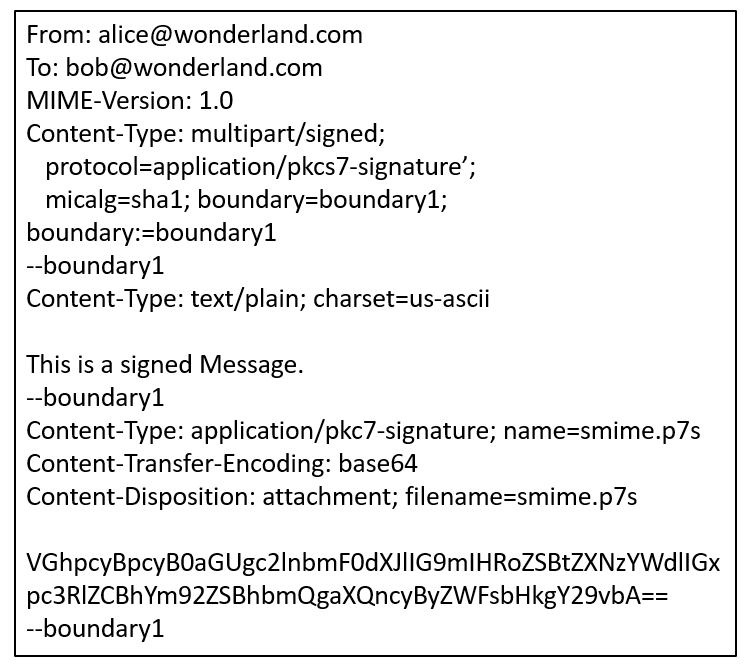
\includegraphics[width=8cm]{images/MIMESignExample.png}
	\centering
	\caption{Exemple du format MIME}
	\label{fig:MIMEExemple}
\end{figure}

Dans ce contexte S/MIME vient ajouter un type MIME \textit{application/pkcs7-mime}, un format de données, qui fabrique une enveloppe chiffrée d'une entité MIME. Pour les signatures S/MIME utilisera plus les signatures détachées et le type \textit{multipart/signed} pour cela ou encore \textit{application/x-pkcs7-signature}. Anciennement, c'était effectivement le format de message PKCS\#7 utilisé pour le format des messages chiffrés. Cependant, à l'heure actuelle c'est la spécification de CMS (Cryptographic Message Syntax) qui est utilisé dans ces types S/MIME. La Figure \ref{fig:SMIME_Encapsulation} permet de mieux se représenter cette encapsulation avec l'objet CMS \textit{SignedData}, inspiré d'un cours de la Haute École de Rapperswill\footnote{\url{http://security.hsr.ch/lectures/Internet_Security_1/07-SecureEmail.pdf}}

\begin{figure}[h!]
	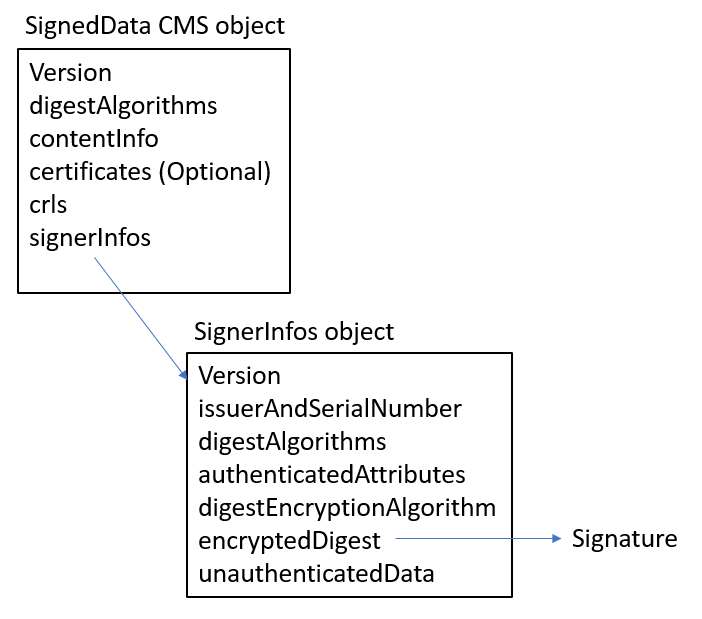
\includegraphics[width=8cm]{images/MIMESignerDataExample.png}
	\centering
	\caption{Encapsulation des données avec S/MIME}
	\label{fig:SMIME_Encapsulation}
\end{figure}

Afin de commencer à signer des messages avec S/MIME et pouvoir recevoir des messages chiffrés il faut un certificat. Ce certificat peut être obtenu soit par une autorité de certification interne ou une autorité externe. Ces certificats peuvent être de classe 1 (vérification que le propriétaire du certificat peut recevoir des messages envoyés au "From:" de ses messages) ou de classe 2 avec plus de précisions sur le propriétaire du certificat.

Pour signer un message, S/MIME va utiliser la clé privée liée au certificat de la source, ainsi le message va être signé avec la primitive adéquate par rapport aux informations du certificat. Puis la signature sera envoyée avec le certificat, afin que le destinataire puisses vérifier la signature à l'aide du certificat, et vérifier le certificat avec un CA.

Comme le présente la RFC8551~\cite{RFC8551}, le chiffrement effectué par S/MIME s'approche de celui fait par PGP, en effet S/MIME va chiffrer la clé de chiffrement symétrique (Content Encryption Key dans CMS) une fois par destinataire en utilisant la clé publique authentifiée par leur certificat respectif et aussi une fois pour la source du message (afin de pouvoir relire le message envoyé à l'avenir). Les algorithmes qui doivent être pris en charge dans CMS sont les suivants selon la RFC8551 dans la table \ref{table:refSMIMEAlgos}.

\begin{table}[h!]
	\centering
	\caption{Table des algorithmes utilisés par S/MIME}
	\label{table:refSMIMEAlgos}
	\begin{adjustbox}{width=\textwidth}
		\begin{tabular}{||c c c c||}
			\hline
			Symetric & Asymetric & Hash & Signature \\ [0.5ex]
			\hline\hline
			AES-128 CBC & ECDH sur P-256 & SHA-256 & ECDSA (courbe P-256 et SHA-256) \\
			ChaCha20-Poly1305 & ECDH  avec HKDF-256 & SHA-512 & EdDSA (courbe 25519 avec PureEdDSA mode) \\
			AES128-GCM & RSA & & RSA PKCS \#1 v1.5 avec SHA-256 \\
			AES256-GCM & RSAES-OAEP & & RSASSA-PSS avec SHA-256\\
			\hline
		\end{tabular}
	\end{adjustbox}
	
\end{table}
\paragraph*{Propriétés cryptographiques.}
S/MIME est aussi créé pour établir un \textbf{chiffrement bout-en-bout} et ainsi éviter de révéler trop d'informations lors d'une brèche dans un MDA par exemple. 
\textbf{Authentification} et \textbf{intégrité} du message en utilisant la signature digitale, en plus de \textbf{non-répudiation} grâce à celle-ci. Le fait d'avoir le message chiffré de bout en bout permet un certain respect de la vie privée, on ne peut voir les données envoyées.
\paragraph*{Utilisation.}
Pour utiliser S/MIME et avoir des exemples et références de certificats, deux fournisseurs \textbf{gratuits} ont été utilisés pour évaluer les certificats S/MIME.

Tout d'abord, un plugin firefox qui permet d'avoir des certificats pour GMail et envoyer des emails signés et chiffrés à l'aide de S/MIME a été testé. La clé privée est générée par l'extension localement et n'est pas sauvegardée dans un cloud, il est possible de la sécurisé à l'aide d'une \textit{passphrase}. Cependant, les certificats ne sont pas vérifié correctement comme on peut le voir à la réception dans MeSince (le prochain programme testé) à la Figure \ref{fig:SMIME_MeSinceProblem}. Le certificat utilise RSA (algorithme exact non spécifié) avec SHA256 pour la signature des messages.
\begin{figure}[h!]
	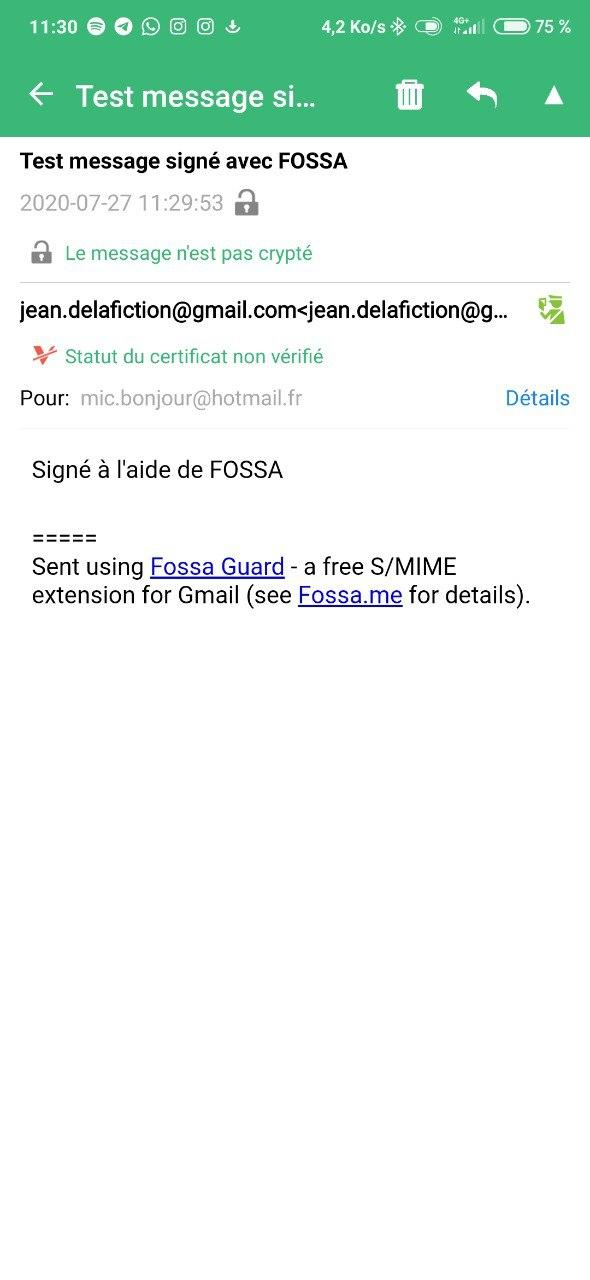
\includegraphics[width=8cm]{images/SMIME_FossaProblem.jpg}
	\centering
	\caption{Erreur de vérification pour Fossa}
	\label{fig:SMIME_FossaProblem}
\end{figure}

Pour tester S/MIME, un compte MeSince\footnote{\url{https://www.mesince.com}} a été utilisé. En effet, ce service permet d'utiliser S/MIME afin de chiffrer et signer ses emails, et ils fournissent les certificats, seulement il ne fonctionnait pas avec Gmail. De plus, le service fourni n'a pas fonctionné pour se connecter et récupérer son certificat, ainsi le certificat a été généré et peut être utilisé par leur application mobile pour envoyer des emails signés et chiffrés, cependant il n'est pas accessible et ne peux donc pas être directement analysé. Sur l'application mobile, il n'y a pas moyen de vérifier la clé générée ni même de l'exporter. Ce service est donc à éviter, de plus on ne manquera pas l'erreur de traduction pour le mot "crypté" qui ne se dit pas en français.

Attention cependant, le même problème avec Fossa arrive comme le montre la Figure \ref{fig:SMIME_MeSinceProblem}. Par contre l'avertissement n'est pas très voyant au sein de Gmail (qui intègre pourtant le support S/MIME dans G Suite). Les certificats utilisent RSA (algorithme exact non spécifié) avec SHA256 pour la signature des messages.

\begin{figure}[h!]
	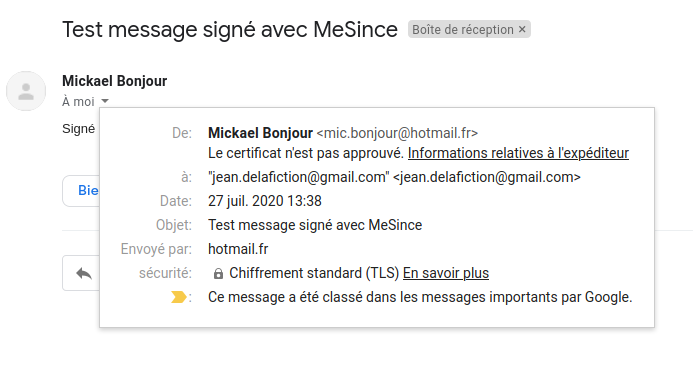
\includegraphics[width=15cm]{images/mesince_problem.png}
	\centering
	\caption{Erreur de vérification pour MeSince}
	\label{fig:SMIME_MeSinceProblem}
\end{figure}

MeSince informe que la clé privée est automatiquement sauvegardée dans leur cloud sécurisé, ce qui n'est pas forcément une bonne nouvelle (fuite de leur cloud, cloud dont ils ont accès). De plus, la clé est générée automatiquement, donc aucune vérification de la part de l'utilisateur ne peut être faite.

Cependant, ces deux tests effectués ne représentent pas vraiment une utilisation réelle de S/MIME, en effet, le meilleur moyen de tester S/MIME aurait été d'avoir un nom de domaine à soi et de générer des certificats S/MIME pour une adresse privée. Ensuite, il faudra importer manuellement ses certificats et ses clés dans le client mail utilisé.

\section{Implémentations existantes}
Dans cette section, certaines implémentations des protocoles discutés dans la section précédente sont analysés, particulièrement ceux implémentant PGP.

\subsection{Protonmail}

\paragraph*{Revendications.}
Protonmail revendique beaucoup de propriétés cryptographiques, telles que le zero-access encryption (lors de la réception d'un message externe chiffré ou non Protonmail le chiffrera avec la clé publique de l'utilisateur pour ne plus y avoir accès dans le futur). Et le chiffrement de bout-en-bout pour les messages sécurisés, cela même avec leur fonctionnalité de chiffrement vers l'extérieur utilisant AES256-GCM. Mettre une date d'expiration sur un email est aussi possible, afin que le destinataire ne puisse le lire que dans un temps imparti.

Pour l'authentification Protonmail utilise une manière fortement sécurisée (SRP) pour ne pas avoir d'informations directes sur le mot de passe de l'utilisateur.

Protonmail chiffre automatiquement les emails d'un utilisateur Protonmail à un autre via PGP.
\paragraph*{Fonctionnement.}
Protonmail a plusieurs modes de fonctionnement dépendant du destinataire final. En effet de Protonmail à Protonmail les emails sont chiffrés à l'aide de PGP automatiquement. On peut utiliser Protonmail pour utiliser PGP si on a la clé de notre destinataire par exemple. Et on peut écrire un email chiffré à quelqu'un qui n'utilise pas PGP grâce à une fonctionnalité de chiffrement vers l'extérieur.

Cette fonctionnalité enverra une URL au destinataire qui, en la consultant, pourra déchiffrer l'email en utilisant un mot de passe communiqué auparavant de manière sécurisée entre les deux parties. Un exemple d'email utilisant cette fonctionnalité est présenté dans la Figure \ref{fig:ProtonmailPres}.

\begin{figure}[h!]
	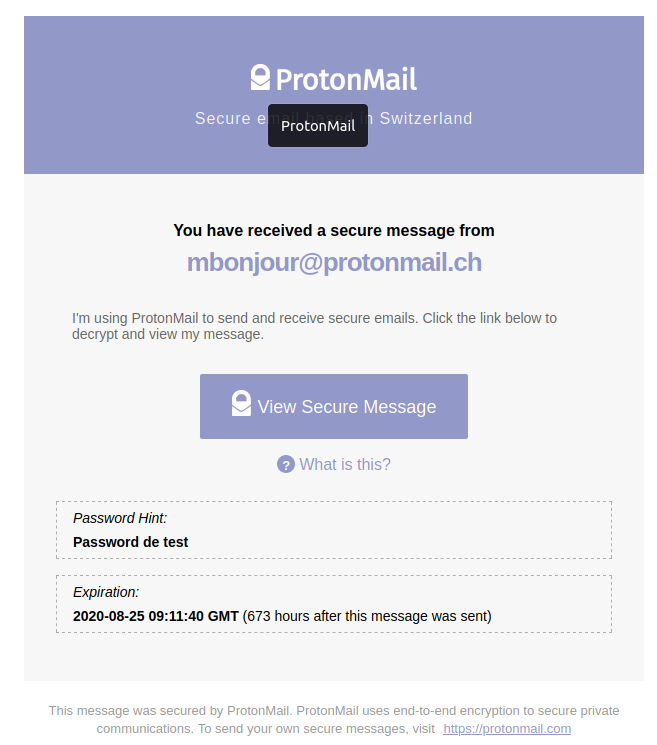
\includegraphics[width=10cm]{images/protonmailPresentation.png}
	\centering
	\caption{Présentation d'un email chiffré Protonmail}
	\label{fig:ProtonmailPres}
\end{figure}

\paragraph*{Open Source.}
Leur code est open-source afin d'avoir une validation externe, de plus ils ont un programme de Bug Bounty pour les chercheurs. Ils ont largement contribué au projet d'intégration openpgp, en javascript et en Go.

\paragraph*{Utilisation.}
Lors de l'utilisation de protonmail, l'analyse des clés PGP générées a montré qu'elles utilisent RSA. Pour envoyer ou recevoir des messages via PGP, Protonmail le fait de manière très transparente. Apparemment en utilisant les mêmes serveurs de clés cités plus haut pour Enigmail. En effet, les deux comptes mails de tests ont pu s'envoyer des messages sans s'envoyer leurs clés publiques au préalable.

Un mot de passe supplémentaire est utilisé pour chiffrer notre boite mail, afin de protéger les emails si une brèche survenait au niveau du stockage Protonmail. De plus, la technologie utilisée pour l'authentification et les mots de passe est SRP (Secure Remote Password). Permettant de ne pas avoir de \textit{hashs} de mots de passe stockés chez Protonmail.

Par contre, la génération de la clé privée à la création du compte est assez obscure mais de l'information est disponible sur le site de Protonmail\footnote{\url{https://protonmail.com/support/knowledge-base/how-is-the-private-key-stored/}}.

\paragraph*{Critiques.}
Protonmail est très critiqué de manière générale sur les réseaux sociaux. De plus une réponse\footnote{\url{https://protonmail.com/blog/cryptographic-architecture-response/}} au chercheur Nadim Kobeissi~\cite{journals/iacr/Kobeissi18a} avait été formulée par Protonmail suite à son papier sur l'insécurité de leur webmail. Cependant, ils sont surtout critiqués sur les réseaux sociaux par des chercheurs en sécurité\footnote{\url{https://twitter.com/FiloSottile/status/1277068367728435202}} pour leur publicité mensongère, en effet, leur page d'accueil indiquait une sécurité pour \textbf{tous} les emails sortants. Ce qui n'est pas le cas, uniquement les emails intentionnellement chiffrés à l'aide de PGP ou chiffrés vers l'extérieur sont effectivement chiffrés. L'annonce ne représentait donc pas la réalité, ce qui peut être mal interprété par les utilisateurs. Après vérification, la page d'accueil a bien été modifiée pour ne plus inclure la mention de chiffrement automatique pour tous les emails. Le commentaire fait référence aussi à d'autres points :
\begin{itemize}
	\item Ingère les emails en plaintext - par rapport à leur politique de zero-access, ils ont au moins une fois accès au plaintext d'un email non chiffré.
	\item Pas de réelles solutions pour du chiffrement vers l'extérieur - La solution amenant l'utilisateur distant à se connecter à leur service pour déchiffrer un message n'est pas une solution viable.
	\item Utilise de la cryptographie dans le navigateur non validée - Modules cryptographiques servis par les serveurs de Protonmail, on revient ici aux revendications de ce papier~\cite{journals/iacr/Kobeissi18a}. Malgré cela une solution existe désormais, utiliser un bridge disponible sur github\footnote{\url{https://github.com/ProtonMail/proton-bridge}}.
	\item Agit comme un serveur de clés, sans transparence de clés - Suite à la mise en place d'un serveur de clés pour chercher les clés PGP d'utilisateur Protonmail pas de transparence sur ce serveur n'a été communiqué.
\end{itemize}
\subsection{Tutanota}
\paragraph*{Fonctionnement.}
Tutanota est un client mail sécurisé, il permet de chiffrer les emails vers l'extérieur. Cela en utilisant AES128-CBC (selon analyse du code source\footnote{\url{https://github.com/tutao/tutanota/blob/master/src/api/worker/crypto/Aes.js}}). Mais aussi RSA-OAEP pour chiffrer les communications entre deux utilisateurs Tutanota\footnote{\url{https://tutanota.com/fr/security/}}.
\paragraph*{Utilisation.}
L'utilisation de Tutanota est facile, en effet Tutanota utilise le même principe que Protonmail pour le chiffrement vers l'extérieur. En chiffrant l'email et en le gardant sur ses serveurs puis en envoyant un email au destinataire comme celui présenté dans la Figure \ref{fig:TutanotaPres}.

\begin{figure}[h!]
	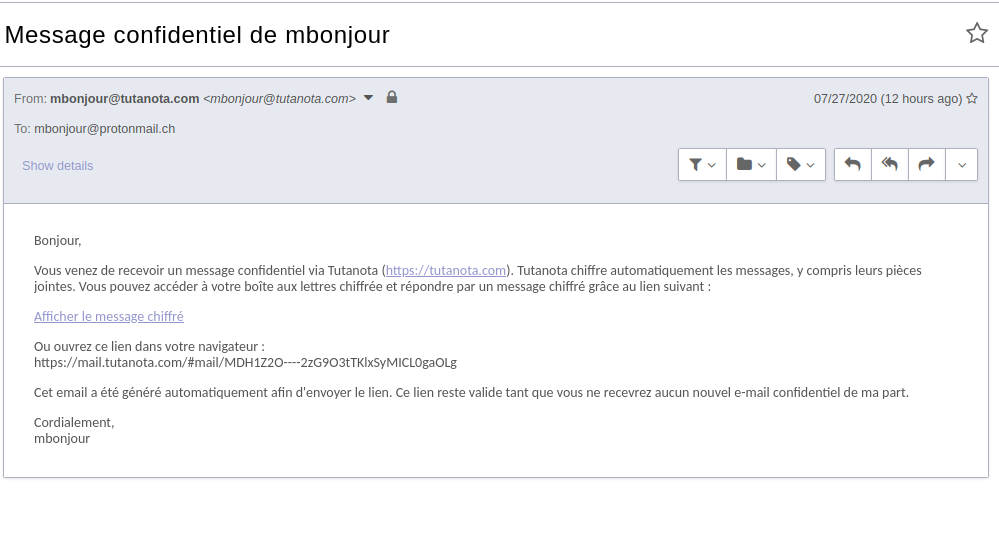
\includegraphics[width=14cm]{images/tutanotaPresentation.png}
	\centering
	\caption{Présentation d'un email chiffré Tutanota}
	\label{fig:TutanotaPres}
\end{figure}

\section{Attaques existantes}
Présentation des attaques faites sur les différents systèmes présentés jusqu'ici ainsi que leur fonctionnement global.
\subsection{Défauts webmails}
Selon un chercheur, l'infrastructure de Protonmail aurait des failles via son webmail~\cite{journals/iacr/Kobeissi18a}. Mais son papier est en fait plus général et parle des webmails en règle générale.

Il part du principe que les serveurs de Protonmail ne sont pas des serveurs à faire confiance, pour ainsi prouver le zero-knowledge de Protonmail. Par contre, le fait qu'ils ne peuvent pas être mis en confiance est un problème selon lui, car c'est ces serveurs qui vont délivrer le code d'OpenPGP afin de faire le chiffrement.

Cela indique que si Protonmail était corrompu le fait d'avoir le code délivré par Protonmail pourrait avoir des effets néfastes. Comme p.ex l'extraction de la clé privée PGP. La conclusion est que dès le moment où vous avez utilisé une fois le webmail de Protonmail la clé PGP pourrait être corrompue ou connue de Protonmail.
\subsection{EFAIL}
\label{attacks:EFAIL}
Malgré ces sécurités qui pourraient être mises en place à l’heure actuelle, une attaque nommée EFAIL~\cite{conf/uss/PoddebniakD0ISF18} a été faite en 2018. En effet, cette attaque a seulement été mitigée en évitant d’afficher les contenus HTML et les images dans les boîtes mails de base. Car le problème vient principalement de là, des problèmes sont liés aussi aux modes de chiffrement utilisé (typiquement CBC et CFB pour S/MIME et PGP respectivement) grâce à des "gadgets". Cette attaque par gadget est démontrée sur le site officiel d'EFAIL\footnote{\url{https://efail.de/}} à l'aide de la Figure \ref{fig:efailAttack}. Ces gadgets sont possible car une partie du texte clair est connue (a), l'attaquant peut ainsi construir un bloc de 0 lorsque déchiffré en manipulant l'IV. La paire $X$ et $C_0$ est appelée un CBC gadget. Ce gadget pourra être utilisé pour pour ajouter du contenu permettant à l'exfiltration du texte clair (c).

\begin{figure}[h!]
	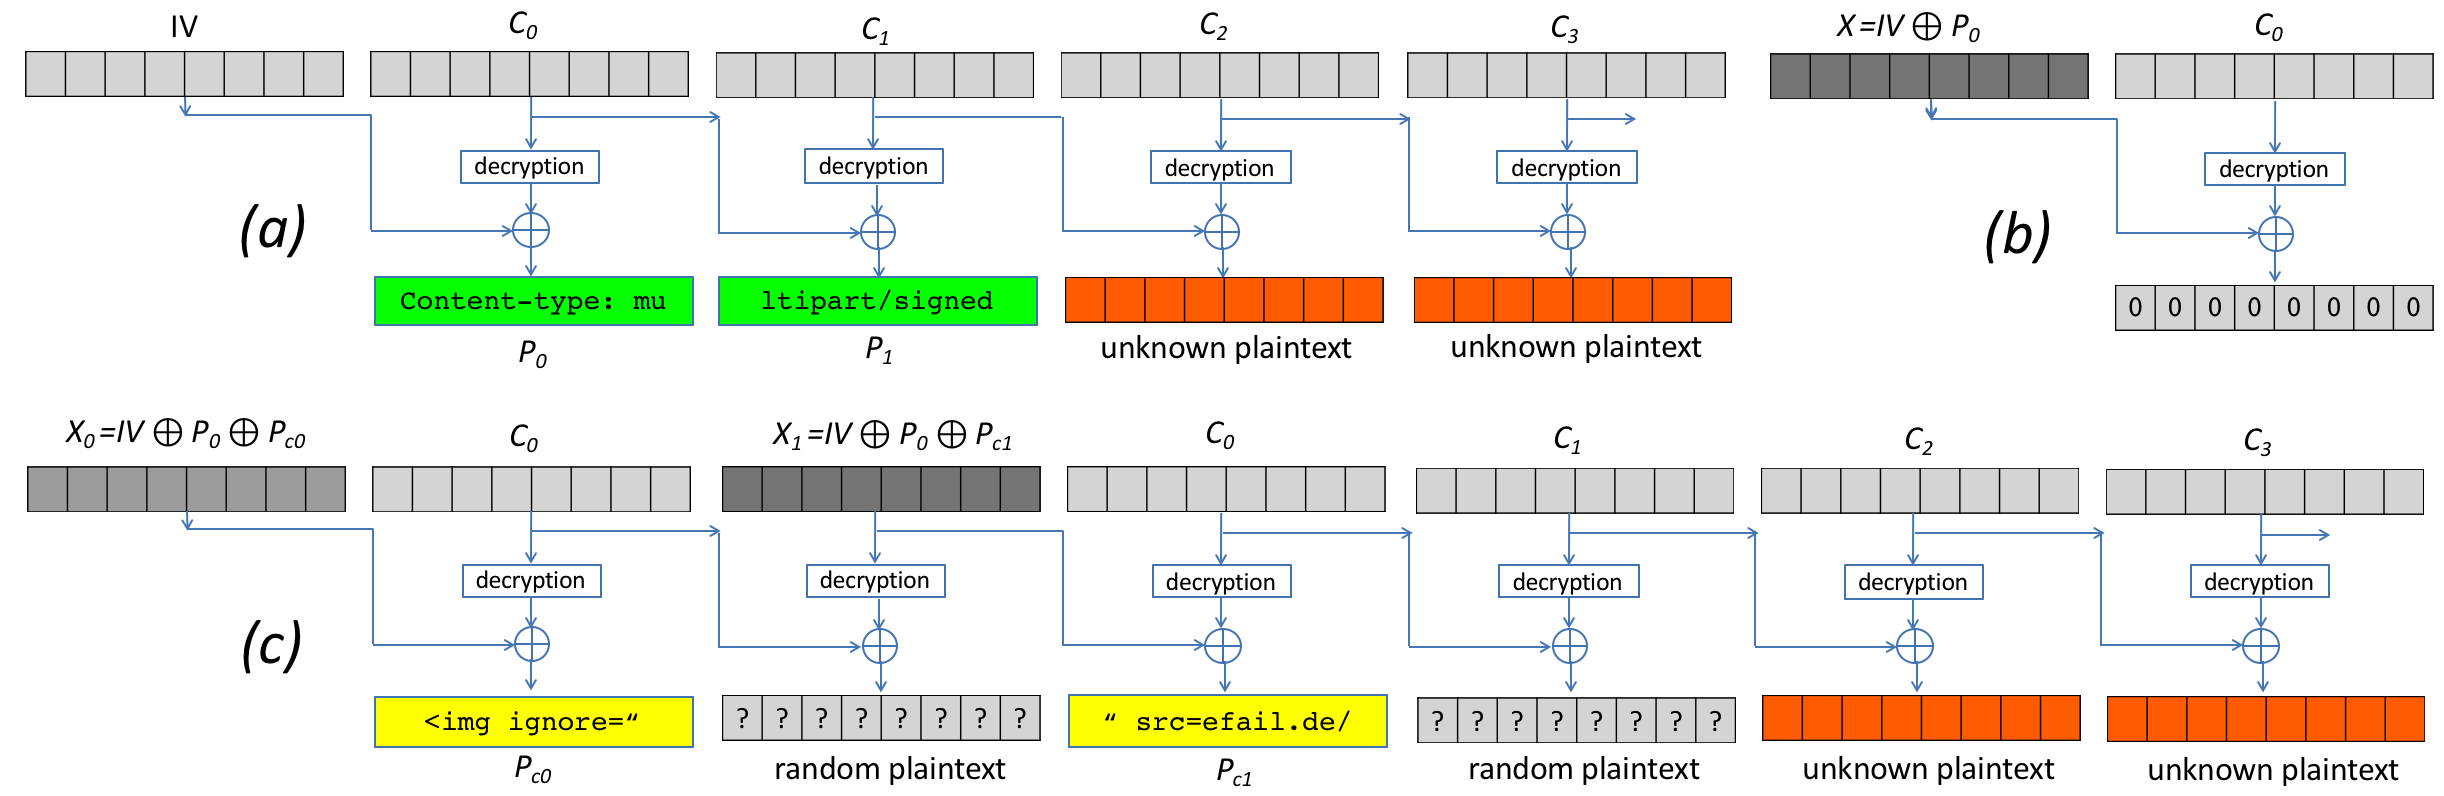
\includegraphics[width=\textwidth]{images/efail-attack.png}
	\centering
	\caption{Attaque par gadgets pour les modes d'opération CFB et CBC}
	\label{fig:efailAttack}
\end{figure}

Cette attaque permet en fait d'injecter une image dans l'HTML du message, puis faire en sorte de récupérer le contenu du message déchiffré dans l'URL. Ceci est possible grâce au multi parties de MIME et en les abusant afin d'entourer le message chiffré d'une balise \textit{img} et de mettre en source le message qui sera déchiffré selon les règles de MIME. Ainsi l'attaquant aura le message déchiffré dans l'URL qu'il peut contrôler. 

Cette attaque exploite en fait une erreur par rapport à la gestion des messages utilisants HTML et multipart/mixed. Il faudrait en effet vérifier dans ces cas que le document HTML est un document entier. Ainsi que de ne pas traiter le contenu chiffré de la même origine que du contenu non protégé. La spécification~\cite{RFC8551} S/MIME a aussi mise à jour pour implémenter des chiffrements authentifiés et remplacer CBC qui permettait des attaques par gadgets.
\subsection{SHA-1 Shambles}
Récemment~\cite{journals/iacr/LeurentP20} une attaque sur SHA-1 avec un préfixe choisi a été démontrée en pratique\footnote{\url{https://sha-mbles.github.io/}}. Cette attaque permet de se faire passer pour un autre utilisateur grâce à une attaque par préfixe choisi sur SHA-1. SHA-1 était en effet l'algorithme de hachage par défaut pour signer les clés d'autres utilisateurs dans le \textit{Web Of Trust} de PGP.

L'attaque fonctionne ainsi pour un l'attaquant, Bob, voulant se faire passer pour Alice: 
\begin{itemize}
	\item Il va générer deux clés PGP à l'aide de l'attaque par préfixe choisi, une clé A contenant une grande clé publique mais qui sera facilement factorisable avec l'identité d'Alice puis une clé B contenant une petite clé publique ainsi que l'identité de Bob au sein d'un objet JPEG, et après la fin de ce format l'identité d'Alice "cachée". Le fait de générer ces deux clés avec l'attaque permet d'avoir un hash commun pour les deux clés publiques $H(A) = H(B)$.
	\item Bob va donner sa clé publique à d'autre utilisateurs et demander de la signer (clé tout à fait correcte à première vue).
	\item Il va pouvoir utiliser les signatures effectuées sur sa clé sur la clé A générée auparavant.
	\item Cela a pour effet d'avoir une clé publique contenant l'identité d'Alice qui est signée pas des utilisateurs du \textit{Web Of Trust}. Les autres utilisateurs faisant confiance à ces utilisateurs feront donc confiance à la clé d'Alice alors que c'est une clé forgée.
\end{itemize}
\section{Signal}
L'analyse s'est faite aussi pour la messagerie instantanée à cause de sa ressemblance avec la messagerie électronique. 
\subsection{Fonctionnement}
Le fonctionnement de Signal est complexe à expliquer, ainsi la Figure \ref{fig:signal} sera plus parlante pour expliquer le Diffie-Hellman Ratchet. Ce premier Ratchet permet d'utiliser Diffie-Hellman afin d'avoir une première sortie synchronisée entre l'envoi et la réception d'un utilisateur. Au début de la discussion, Bob va envoyer sa clé publique et Alice va pouvoir commencer son premier Ratchet en générant elle aussi une paire de clés Diffie-Hellman. On verra dans la Figure \ref{fig:signalSecond} ce qu'il se passe ensuite pour le chiffrement des messages mais une fois cette opération finie, Alice envoie sa clé publique précédemment générée à Bob pour qu'il puisse générer la même clé partagée à l'aide de Diffie-Hellman et ainsi déchiffrer le contenu en s'aidant du Deuxième Ratchet.

\begin{figure}[h!]
	\centering
	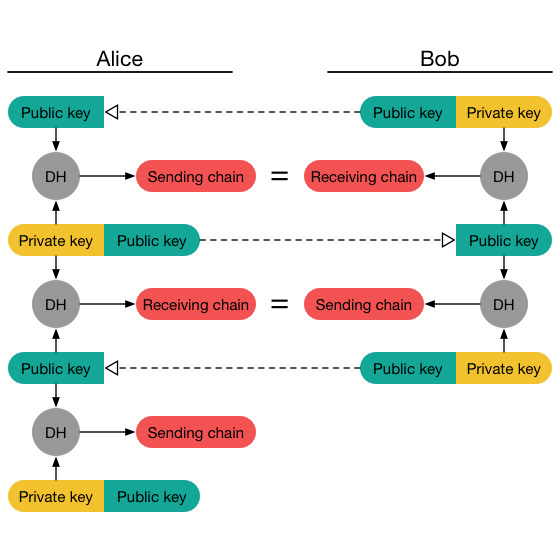
\includegraphics[width=10cm]{images/signalFonctionnement.png}
	\caption{Fonctionnement du DH Ratchet~\cite{doubleratchet}}
	\label{fig:signal}
\end{figure}

Par contre, l'image est une simplification, la clé DH ne va pas être utilisée telle quelle, elle sera insérée dans une KDF avec une Root Key (partagée à l'aide de X3DH) qui sortira la prochaine Root Key et la Receiving/Sending Chain Key qui sera donnée au deuxième Ratchet.

Le deuxième Ratchet (voir Figure \ref{fig:signalSecond}) va générer une clé pour chaque message/batch de messages afin d'envoyer un message chiffré avec le moins d'utilisation de la même clé possible. Ainsi la forward secrecy est plus forte.Dans cet exemple on voit qu'Alice a envoyé un message chiffré à l'aide d'A1 puis qu'elle a reçu un nouveau DH Ratchet de Bob qui lui a permis de générer sa prochaine Receiving Chain Key et de déchiffrer les messages que Bob a envoyés (B1).

\begin{figure}[h!]
	\centering
	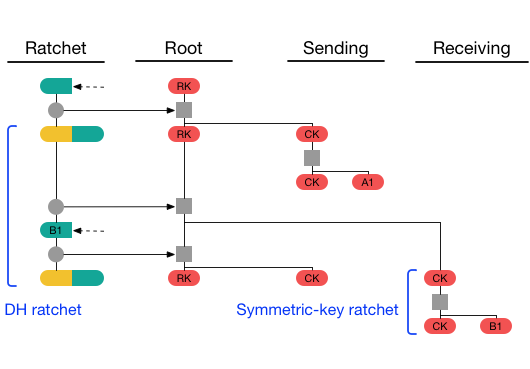
\includegraphics[width=12cm]{images/secondRatchet.png}
	\caption{Fonctionnement du deuxième Ratchet~\cite{doubleratchet}}
	\label{fig:signalSecond}
\end{figure}

\subsection{Propriétés cryptographiques}
Signal a de nombreux avantages concernant les propriétés cryptographiques qu'il promet. En effet le \textit{Double Ratchet} permet de la \textbf{Break-in recovery}, a une \textbf{Perfect Forward Secrecy}, \textbf{End-to-End encryption}, \textbf{Non-Répudiation}.
\subsection{Problèmes d'intégrations}
Le problème avec le protocole Signal quant aux besoins niveaux emails est la \textit{perfect forward secrecy} qui est très forte. En effet, comme vu dans la Section précédente, il utilise une clé par message grâce au \textit{Double Ratchet}. Cependant ce fonctionnement comporte un gros problème en rapport aux emails, en effet si l'on veut pouvoir récupérer les anciens emails reçus/envoyés cela devient vraiment compliqué. La \textit{forward secrecy} est une propriété utile dans un système d'emails, mais il faut pouvoir aussi récupérer les messages facilement si l'on connaît la clé privée. Alors qu'avec ce système de Double Ratchet il nous faudrait enregistrer chaque Diffie-Hellman Ratchet pour reconstruire toute les clés utilisée.
\section{Compromis}
Pour passer à l'implémentation concrète d'un nouveau protocole il faut faire des compromis et aller chercher dans des primitives moins connues.

Je suis tout de même resté sur un système de clés publiques comme PGP le fait. Cependant, cette primitive a une identité propre à chaque clé publique ce qui évite un système de certificat trop complexe comme S/MIME.

De plus, pour avoir une \textit{forward secrecy}, on peut ajouter une notion de temps ou de token à l'ID pour chaque batch de messages comme expliqué plus précisément dans la Section \ref{subsec:pseudoSecrecy}.
\subsection{Résultats des recherches}
Comme mentionné avant, les recherches ont beaucoup été orientées sur le protocole Signal qui a une très bonne forward secrecy et résilience. Cependant, le problème avec l'utilisation des emails, c'est d'avoir envie de consulter tous ses emails depuis n'importe quel appareil. Ce n'est malheureusement pas le cas avec Signal à moins de conserver une \textit{root key} ainsi que tous les diffie-hellman ratchet quelque part qui ferait s'effondrer les caractéristiques principales du protocole.

S/MIME est la solution prédominante pour s'envoyer des emails chiffrés, cependant il est compliqué de l'utiliser. Il est en effet difficile d'obtenir un certificat pour envoyer des emails et échanger avec une autre personne ayant S/MIME. De plus, la complexité d'un système de PKI et l'overhead induit est assez conséquent.

En faisant quelques essais PGP de mon côté, je me suis heurté à beaucoup de difficultés et de problèmes avec les clés PGP. Notamment pour se les échanger, mais pour envoyer un email ensuite ce n'est pas si complexe. Le problème étant de bien voir les primitives utilisées pour chiffrer/signer notre email, en effet, les solutions \textit{plug-and-play like} ne permettent pas une gestion précise des primitives cryptographiques utilisées. Cela pourrait induire à des primitives par défaut non sécurisées, comme l'a démontré EFAIL(c.f. \ref{attacks:EFAIL}).

Dans la Table \ref{tab:recapProps}, on peut voir les différentes implémentations ainsi que les propriétés cryptographiques qu'elles atteignent. On voit surtout que Signal offre plus de possibilités que d'autres systèmes. Tutanota n'offre pas de Forward Secrecy car les mails sont chiffrés à l'aide de RSA-OAEP entres les utilisateurs, les mails vers l'externe chiffré sont sûrement chiffré avec des clés différentes et on peu donc parler de Forward Secrecy. Protonmail utilise PGP entresses utilisateurs et le chiffrement vers l'extérieur est sûrement aussi pseudo forward secure. Tutanota et Protonmail n'offre pas de répudiation à cause de PGP.
% TODO expliquer à la présentation
\begin{table}[]
	\centering
	\begin{tabular}{|lccc|}
		\hline
		Property          & Signal & Protonmail & Tutanota \\ \hline
		Forward Secrecy   & Oui    &            &          \\
		Répudiation       & Oui    &            &          \\
		Non répudiation   &        & Oui        & Oui      \\
		Break-in recovery & Oui    &            &          \\ \hline
	\end{tabular}
	\caption{Récapitulatif des propriétés cryptographiques de différentes implémentations}
	\label{tab:recapProps}
\end{table}
\section{Primitives}
Cette section présente les primitives considérées pour implémenter un système de messagerie sécurisée. Elle contient un aperçu des primitives analysées, pourquoi elle a été ou non retenue et leur fonctionnement en quelques mots.
\subsection{Primitives analysées}
Les primitives analysées sont présentées ci-après. Elles ont en commun de s'appuyer sur un principe basé sur l'identité. C'est très pratique dans un système de email car une identité peut-être très vite définie par le biais d'une adresse email. Voici donc les technologies auxquelles les recherches se sont portées :
\begin{itemize}
	\item Identity based encryption~\cite{conf/crypto/Shamir84}, primitive instaurant en premier le binding entre un ID et le chiffrement, ceci afin d'éviter les infrastructures complexes de PKI. Cependant, cette primitive introduit le \textit{key escrow problem}, un problème inhérent de la construction qui nécessite un KGC générant les clés privées pour les utilisateurs et qui en a par la conséquente connaissance.
	\item A Forward-Secure Public-Key Encryption Scheme~\cite{conf/eurocrypt/CanettiHK03}, cette primitive présente un schéma de \textit{hierarchical identity based encryption} qui permet de restreindre le problème de \textit{key escrow} partiellement. Et la sécurité atteinte est CPA sûre et d'ailleurs moins sécurisée que certains schémas dans le \textit{Random Oracle Model} (expliqué ci-après dans la Sous-Section \ref{subsec:asavoir}). Ils introduisent aussi un concept de Binary Tree Encryption.
	\item Certificateless PKC~\cite{conf/asiacrypt/Al-RiyamiP03}, primitive permettant d'utiliser un système basé sur l'identité. Cependant, elle permet d'éviter le \textit{key escrow problem} de la cryptographie basée sur l'identité.
\end{itemize}
\subsection{Primitive choisie}
- Certificateless PKC~\cite{conf/asiacrypt/Al-RiyamiP03} (souvent nommé CL-PKC dans la suite du document).

 Cette primitive a été choisie car elle est similaire à de l'identity based encryption avec un ID pour désigner une clé publique. Le problème avec l'identity based encryption c'est le fait que le serveur central génère la clé publique et la clé secrète de l'utilisateur, cela amène ce qu'on appelle le \textit{key escrow} problème. C'est le fait qu'une entité connaisse à elle seule toutes les clés de tous les utilisateurs. Ce problème est résolu dans le certificateless en introduisant des \textit{Partial Private Keys} permettant d'avoir une clé secrète partiellement générée par le serveur (KGC - Key Generation Center) et par l'utilisateur puis assemblée pour former la clé privée seulement connue de l'utilisateur. De plus, cette primitive a l'avantage de ne pas introduire de certificats et ainsi évite la complexité d'une infrastructure de PKI (Public Key Infrastructure) tout en \textit{bindant} les clés publiques à un certain ID. Et cela en ayant un niveau de sécurité équivalent à celui accordé à un CA dans une PKI.
\section{Recherches sur la primitive}
\label{sec:primitiveSearch}
Dans cette section je vais introduire les détails techniques et les principes mathématiques utilisés. De plus, le choix du schéma parmi tous ceux analysés est détaillé ici. Ainsi que des précisions sur certains principes introduits par ce schéma.
\subsection{Principes mathématiques}
\label{subsec:mathPairings}
Les variantes de \textit{Certificateless Cryptography} choisies utilisent un concept appelé les \textit{pairings} ou \textit{bilinear map groups} ou \textit{couplages}. Les informations suivantes ainsi que le choix de la librairie découle du livre \textit{Guide to Pairing-Based Cryptography}~\cite{bookPairing}.

Des groupes tels que $\mathbb{G}_1, \mathbb{G}_2, \mathbb{G}_T$ d'un ordre premier \textit{p} pour lesquels il existe un mapping $e : \mathbb{G}_1 \times \mathbb{G}_2 \rightarrow \mathbb{G}_T$ avec les propriétés suivantes :

1. Bilinéarité : $e(g^a, h^b) = e(g, h)^{ab}$ pour tout $(g,h) \in \mathbb{G}_1 \times \mathbb{G}_2$ et $a,b \in \mathbb{Z}$;

2. Non-dégénérescence : $e(g,h) \neq 1_{\mathbb{G}_T} $ tant que $g,h \neq 1_{\mathbb{G}_{1,2}}$;\\
Plusieurs types de Pairings existent :

\begin{itemize}
	\item \textbf{Type 1} : Lorsque $\mathbb{G}_1 = \mathbb{G}_2$;
	\item \textbf{Type 2} : Lorsque $\mathbb{G}_1 \ne \mathbb{G}_2$ mais qu'un isomorphisme $\phi : \mathbb{G}_1 \rightarrow \mathbb{G}_2$ est connu, mais pas dans l'autre direction.
	\item \textbf{Type 3} : Lorsque $\mathbb{G}_1 \ne \mathbb{G}_2$ et qu'aucun isomorphisme est connu entre $\mathbb{G}_1$ et $\mathbb{G}_2$, dans n'importe quelle direction.
\end{itemize}
Les différents schémas analysés utilisent souvent les pairings de Type 1, cependant la courbe utilisée et RELIC me permet de faire des pairings de Type 3. Une conversion est faite dans les schémas choisis comme vu ci-après. En effet, les pairings de Type 3 sont des pairings plus efficients avec des courbes plus petites tandis que les pairings de type 1 étaient plus utilisés dans les débuts de la \textit{Pairing Based Cryptography}.
\subsection{Notations}
\label{subsec:asavoir}
Avant d'analyser les différents schémas, il faut connaître certaines notions présentes dans les tableaux comparatifs afin de mieux les comprendre. Liste non exhaustive de ces notions et de leurs significations est faite ici.

\paragraph*{Types.} 
Les types présentés peuvent être soit \textbf{concret} soit \textbf{générique}. Les types concrets sont des schémas qui présentent leurs algorithmes en utilisant des calculs bien établis et présentent l'entierté du fonctionnement de leurs schémas, tandis que les schémas présentés génériques peuvent s'appuyer sur d'autres problèmes et se baser sur des algorithmes déjà existants.

\paragraph*{Modèle de sécurité.} 
Ces modèles définissent sur quoi le schéma va se reposer pour établir sa sécurité et comment il va l'évaluer face à un adversaire. À nouveau, il existe deux modèles présents dans les schémas analysés, le \textit{Random Oracle Model} et le \textit{Standard Model}. Le \textit{Random Oracle Model} se base sur des oracles aléatoires mais est un peu controversé. En effet, l'aléatoire cryptographiquement sûr est difficile à atteindre, ainsi habituellement le \textit{Random Oracle Model} implémente ces oracles via des fonctions de hachage. Le modèle standard se base lui sur des problèmes mathématiquement difficiles tel que DDH (Decisional Diffie Hellman).

\paragraph*{Modèle d'adversaires.}
Pour évaluer les schémas de certificateless public key cryptography il y a différents niveaux de sécurité établis pour deux types d'adversaires différents. Ces adversaires ont été décrits dans le papier d'Al-Riyami-Paterson~\cite{conf/asiacrypt/Al-RiyamiP03} pour la première fois afin de prouver que leurs schémas était IND-CCA sûr dans le modèle Standard. Ces deux adversaires ont été défini comme suit :

\begin{itemize}
	\item Type I (\textit{outsider adversaries}) est permis de remplacer des clés publiques, obtenir des clés partielles privées, et des clés privées puis faire des requêtes de déchiffrements.
	\item Type II (\textit{honest but curious KGC}). L'adversaire de Type II est en fait un KGC connaissant la Master Secret Key et qui peut donc générer des PPK, obtenir des clés privées et faire des requêtes de déchiffrement tout en faisant confiance à ce KGC pour ne pas qu'il remplace des clés publiques.
	\item Malicious but passive KGC - KGC ayant la possibilité d'extraire les clés partielles et regarder les textes chiffrés et essayer de les déchiffrer, sans pouvoir extraire la valeur secrète de l'utilisateur ou remplacer sa clé publique. Cependant ce KGC fera le \textit{Setup} de manière honnête.
\end{itemize}

Pour chacun des types d'adversaires, il existe différents niveaux de sécurité comme défini dans le livre \textit{Introduction to Ceritifcateless Cryptography}~\cite{bookIntroCertificateless}.
\subsection{Schémas Certificateless de Chiffrement}
Pour choisir parmi les nombreux schémas existants en certificateless pour le chiffrement j'ai établi un tableau comparatif des différentes manières de faire, inspiré de~\cite{bookIntroCertificateless}. En suivant ce tableau, je me suis rendu compte que la construction de Dent-Libert-Paterson~\cite{conf/pkc/DentLP08} était probablement la plus adaptée en vue des propriétés qu'elle présentait. Le tableau se trouve en annexe \ref{ch:fichiers}.

\subsection{Détails techniques}
Les détails techniques sur le chiffrement avec la \textit{Certificateless Cryptography} sont présentés ci-après. Afin de faire la liaison avec l'implémentation, le code C montrant l'implémentation de chaque algorithme est listé. Ce code est simplifié pour ne pas inclure la création des différents éléments, il est là uniquement pour montrer comment les calculs ont été effectués et non comment la mémoire a été allouée.

Le chiffrement se base sur le problème difficile \textit{The Decision 3-Party Diffie-Hellman Problem} (3-DDH), décider si $T =g^{abc}$ ayant $(g^a, g^b, g^c, T) \in \mathbb{G}_4$.

Pour expliquer les détails techniques, je vais ici montrer les calculs faits dans le schéma choisi~\cite{conf/pkc/DentLP08} et les expliquer. Cependant, dans~\cite{conf/pkc/DentLP08} les pairings symétriques sont utilisés (c.f. Section \ref{subsec:mathPairings}) mais il est mentionné que l'adaptation à des pairings asymétriques est triviale, c'est donc les pairings asymétriques qui seront utilisés. De plus,~\cite{conf/pkc/DentLP08} utilise un groupe multiplicatif, ainsi la conversion vers un groupe additif (car l'implémentation utilise des courbes elliptiques) est faite. Cela facilite la lecture avec l'implémentation faite :

\textbf{Setup($1^k, n$) :} Avec $\mathbb{G}_1, \mathbb{G}_2, \mathbb{G}_T$ avec un ordre $p > 2^k$. $g$ est un générateur de $\mathbb{G}_1$. Ensuite  $g_1 = g \cdot \gamma$ pour un $\gamma \leftarrow  \mathbb{Z}_p^*$ aléatoire. Puis $g_2 \leftarrow \mathbb{G}_2$. Deux vecteurs (U,V) seront tirés aléatoirement dans $\mathbb{G}_2^{n+1}$ en tant que fonctions de hash notés :
\[F_u(ID) = u' \sum_{i=1}^{n} u_j^{i_j}\quad\mathrm{and}\quad F_v(w) = v' \sum_{i=1}^{n} v_j^{w_j}\]
On va aussi prendre une fonction de hash résistante aux collisions : $H : \{0,1\}^* \rightarrow \{0,1\}^n$. Au final notre $mpk$ (master public key) est :
\[mpk \leftarrow (g, g_1, g_2, U, V)\]
Et le $msk$ (master seret key) est $msk \leftarrow g_2 \cdot \gamma$.

\begin{sourcebox}{C}{Fonction de setup}
	void setup(int k, encryption_mpk* mpkSetup, g2_t* msk){
		// g = generator of G1
		g1_get_gen(mpkSetup->g);
		g1_get_ord(p);
		
		// gamma = random from Zp
		bn_rand_mod(gamma, p);
		// g1 = gamma*g
		g1_mul(mpkSetup->g1, mpkSetup->g, gamma);
		// g2 = generator of G2
		g2_get_gen(mpkSetup->g2);
		
		g2_get_ord(p);
		// Generate 2 arrays with G2 elements for the U and  vectors
		for(int i =0; i < MESSAGE_SPACE; ++i){
			bn_rand_mod(uvGen,p);
			g2_mul(mpkSetup->u[i], mpkSetup->g2, uvGen);
			bn_rand_mod(uvGen,p);
			g2_mul(mpkSetup->v[i], mpkSetup->g2, uvGen);
		}
		
		// The master secret key is msk = gamma*g2
		g2_mul(*msk, mpkSetup->g2, gamma);
	}
\end{sourcebox}

\textbf{Extract($mpk, \gamma, ID$) :} On prend $r \leftarrow \mathbb{Z}_p^*$ puis on retourne $d_{ID} \leftarrow (d_1, d_2) = (g_2 \cdot \gamma + F_u(ID) \cdot r, g \cdot r)$

\begin{sourcebox}{C}{Code pour l'extraction}
	void extract(encryption_mpk mpk, g2_t msk, char* ID, encryption_ppk* partialKeys){
		// r random from Zp
		bn_rand_mod(r,p);
		
		// Computes d1 = msk + r*Fu(ID)
		g2_t temp;
		g2_null(temp)
		g2_new(temp)
		
		F(ID, mpk.u, &temp, strlen(ID));
		g2_mul(temp, temp, r);
		g2_add(partialKeys->d1, msk, temp);
		
		// Computes d2 = r*g
		g1_mul(partialKeys->d2, mpk.g, r);
	}
\end{sourcebox}

\textbf{SetSec($mpk$) :} Retourne un secret aléatoirement choisi $x_{ID} \leftarrow \mathbb{Z}_p^*$.

\begin{sourcebox}{c}{Construction de la valeur secrète}
	void setSec(bn_t* x){
		g1_get_ord(p);
		bn_rand_mod(*x, p);
	}
\end{sourcebox}

\textbf{SetPub($x_{ID}, mpk$) :} Retourne $pk_{ID} \leftarrow (X,Y) = (g \cdot x_{ID}, g_1 \cdot x_{ID})$.

\begin{sourcebox}{c}{Fonction de construction pour la clé publique}
	void setPub(bn_t x, encryption_mpk mpkSession, encryption_pk* PKtoGen){
		g2_mul(PKtoGen->X, mpkSession.g2, x);
		g1_mul(PKtoGen->Y, mpkSession.g1, x);
	}
\end{sourcebox}

\textbf{SetPriv($x_{ID}, d_{ID}, mpk$) :} On choisit $r' \leftarrow \mathbb{Z}_p^*$ puis on reprends $(d_1, d_2) \leftarrow d_{ID}$ et on va prendre en secret key : 

\[sk_{ID} \leftarrow (s_1, s_2) = (d_1 \cdot x_{ID} + F_u(ID) \cdot r', d_2 \cdot x_{ID} + g \cdot r')\]
Avec $sk_{ID}$ étant la clé secrète de l'utilisateur, donnée par l'Extract (notre Partial Private Key) est la valeur secrète de SetSec.

\begin{sourcebox}{c}{Création de la clé privée}
	void setPriv(bn_t x, encryption_ppk d, encryption_mpk mpk, char* ID, encryption_sk* secretKeys){
		bn_rand_mod(r, p);
		
		// Computes s1 = x*d1 + r*Fu(ID)
		g2_t pointTemp;
		g2_null(pointTemp)
		g2_new(pointTemp)
		
		g2_mul(secretKeys->s1,d.d1, x);
		F(ID, mpk.u, &pointTemp, strlen(ID));
		g2_mul(pointTemp, pointTemp, r);
		g2_add(secretKeys->s1, secretKeys->s1, pointTemp);
		
		// Computes s2 = x*d2 + r*g
		g1_t temp;
		g1_null(temp)
		g1_new(temp)
		
		g1_mul(secretKeys->s2, d.d2, x);
		g1_mul(temp, mpk.g, r);
		g1_add(secretKeys->s2, secretKeys->s2, temp);
	}
\end{sourcebox}

\textbf{Encrypt($m, pk_{ID}, ID, mpk$) :} Pour chiffrer $m \in \mathbb{G}_T$, on va reprendre $(X,Y) \leftarrow pk_{ID}$. Pour chiffrer ce message on va tirer aléatoirement $s \leftarrow \mathbb{Z}_p^*$ puis calculer : 
\[C = (C_0, C_1, C_2, C_3) \leftarrow (m + e(Y, g_2) \cdot s, g \cdot s,F_u(ID) \cdot s, F_v(w) \cdot s )\]
Où $w \leftarrow H(C_0,C_1, C_2, ID, pk_{ID})$.

\begin{sourcebox}{C}{Code pour le chiffrement}
	void encrypt(gt_t m, encryption_pk pk, unsigned char* ID, encryption_mpk mpk, cipher* c){
		bn_rand_mod(s, p);
		// Computes C0 = e(Y,g2)^s*m
		gt_t temp;
		gt_null(temp)
		gt_new(temp)
		pc_map(temp, pk.Y, mpk.g2);
		gt_exp(temp, temp, s);
		gt_mul(c->c0, m, temp)
		gt_free(temp)
		
		// Computes C1 = s*g
		g1_mul(c->c1, mpk.g, s);
		
		// Computes C2 = s*Fu(ID)
		g2_t pointTemp;
		g2_null(pointTemp)
		g2_new(pointTemp)
		F(ID, mpk.u, &pointTemp, strlen(ID));
		g2_mul(c->c2, pointTemp, s);
		g2_free(pointTemp)
		
		// Computes C3 = s*Fv(w) où w = C0, C1, C2, ID, PK.x, PK.y
		g2_t pointTemp2;
		g2_null(pointTemp2)
		g2_new(pointTemp2)
		
		// Construction of the w bytes object to hash
		// ...
		
		F(w, mpk.v, &pointTemp2, c0size + c1Size + c2Size + strlen(ID) + pkXSize + pkYSize);
		g2_mul(c->c3, pointTemp2, s);
	}
\end{sourcebox}

\textbf{Decrypt($C, sk_{ID}, mpk$) :} On peut reprendre $(C_0,C_1,C_2,C_3) \leftarrow C$ est la clé privée $(s_1, s_2) \leftarrow sk_{ID}$. Afin d'accélérer le déchiffrement le calcul suivant peut être fait en tirant une valeur aléatoire $\alpha \leftarrow \mathbb{Z}_p^*$ :
\[m = C_0 + \frac{e(s_2 + \alpha \cdot g, C_2 ) \cdot e(\alpha \cdot g, C_3)}{e(C_1, s_1 + F_u(ID) \cdot \alpha + F_v(w) \cdot \alpha)}\]
Qui donnera $m$ le texte en clair si le chiffré était bien formaté ou un élément aléatoire dans $G_T$.

\begin{sourcebox}{C}{Code pour le déchiffrement}
	void decrypt(cipher c, encryption_sk sk, encryption_pk pk, encryption_mpk  mpk, char* ID, gt_t* m){
		bn_rand_mod(alpha, p);
		// Construction of the w bytes object to hash (e(Ppub, Qa)*e(U, H2(m,ID,PK,U))*e(Ppub, H3(m,ID,PK)))
		// ...
		// Constructs our point
		F(w, mpk.v, &pointFv, c0size + c1Size + c2Size + strlen(ID) + pkXSize + pkYSize);
		F(ID, mpk.u, &pointFu, strlen(ID));
		
		// m = numerateur * numerateur2 / denominateur
		// alphaG = alpha * g
		g1_mul(alphaG, mpk.g, alpha);
		g1_add(tempNumerateur, sk.s2, alphaG);
		// numerateur = e(s2 + alphaG, C2)
		pc_map(numerateur, tempNumerateur, c.c2);
		// numerateur2 = e(alphaG, C3)
		pc_map(numerateur2, alphaG, c.c3);
		gt_mul(numerateur, numerateur, numerateur2);
		
		g2_mul(pointFu, pointFu, alpha);
		g2_mul(pointFv, pointFv, alpha);
		
		g2_add(Fpoints, sk.s1, pointFu)
		g2_add(Fpoints,Fpoints, pointFv)
		pc_map(denominateur, c.c1, Fpoints);
		
		gt_inv(denominateur, denominateur);
		gt_mul(*m, numerateur, denominateur);
		gt_mul(*m, c.c0, *m);
	}
\end{sourcebox}

\subsection{Schémas Certificateless de Signature}
Pour choisir parmi les nombreux schémas certificateless pour la signature, j'ai établi un tableau comparatif des différentes manières,de faire, inspiré de~\cite{bookIntroCertificateless}. En analysant les différentes possibilités dans ce tableau, il y a peu de solutions qui se dégagent, en effet, on peut voir que beaucoup de schémas de signature sont cassés. Mon choix s'est porté au final sur la construction de Zhang et Zhang~\cite{conf/acns/ZhangWXF06} pour des signatures robustes en Certificateless. J'ai pris cette construction car elle est résistante au Malicious KGC (si le KGC a été setup avec des paramètres vulnérables) datant de 2006 et n'a pas été cassée depuis. Le tableau se trouve en Annexe \ref{ch:fichiers}.
\subsection{Détails techniques}
Là encore, le code C montrant l'implémentation de chaque algorithme est listé. Ce code est simplifié pour ne pas inclure la création des différents éléments, il est là uniquement pour montrer comment les calculs ont été effectués et non comment la mémoire a été allouée.
 
La signature se base sur le problème difficile \textit{The Computational Diffie-Hellman Problem} (CDH). 

Ayant $P, aP, bP$ où $a,b$ aléatoires $\in \mathbb{Z}_q^*$ il n'est pas possible de trouver $abP$.

Pour expliquer les détails techniques, je vais ici montrer les calculs faits dans le schéma choisi~\cite{conf/acns/ZhangWXF06} et les expliquer. Cependant dans~\cite{conf/acns/ZhangWXF06} les pairings sont de type symétriques (c.f. Section \ref{subsec:mathPairings}), les pairings utilisés dans l'implémentation sont de type asymétriques.

\textbf{Setup($1^k $) :} Tout d'abord on va prendre les groupes d'ordre $q$ énoncés auparavant. Puis on choisit un générateur $P \in \mathbb{G}_1$. La \textit{master secret key} va être choisie aléatoirement $s \in \mathbb{Z}_q^*$. Puis la clé publique calculée : $P_{pub} = sP$. Finalement, trois fonctions de hash distinctes $H_1, H_2, H_3$ vont être choisies, chacune d'elle \textit{mappant} de $\{0,1\}^*$ à $\mathbb{G}_2$. Pour cela j'ai choisi de faire du \textit{Hash Domain Separation} comme expliqué dans le Chapitre \ref{ch:impl}. On défini les $\mathbf{params} = (\mathbb{G}_1,\mathbb{G}_2,\mathbb{G}_T,e,q,P,P_{pub},H_1,H_2,H_3)$

\begin{sourcebox}{C}{Code C pour le Setup}
	void setupSig(int i, signature_mpk *mpk, bn_t *s){
		// q = Order of G1
		g1_get_ord(q);
		
		// s = random Zq
		bn_rand_mod(*s, q);
		
		// Choose a generator P
		g1_get_gen(mpk->P);
		// Setup Ppub = s*P
		g1_mul(mpk->Ppub, mpk->P, *s);
	}
\end{sourcebox}

\textbf{Partial-Private-Key-Extract($params, s, ID_A$) :} Pour avoir la \textit{Partial Private Key} ($D_A$) de l'user $A$ avec l'identité $ID_A$. Calculer $Q_A = H_1(ID_A)$. Alors $D_A = sQ_A$.

L'utilisateur peut vérifier sa clé partielle à la réception en vérifiant cette équation : $e(P, D_A) = e(Ppub, Q_a)$.

\begin{sourcebox}{C}{Code C pour l'extraction de la clé partielle privée}
	void extractSig(signature_mpk mpk, bn_t msk, char* ID, signature_ppk * partialKeys) {
		// Qa = H1(ID)
		g2_map(qa, ID, strlen(ID));
		// D = msk*Qa
		g2_mul(partialKeys->D, qa, msk);
		
		// Vérification de la clé privée partielle
		pc_map(test1, mpk.P, partialKeys->D);
		pc_map(test2, mpk.Ppub, qa);
		
		if (gt_cmp(test2, test1) == RLC_EQ) {
			printf("The partial private key extraction is correct !\n");
		}
	}
\end{sourcebox}

\textbf{Set-Secret-Value :} La valeur secrète $x \in \mathbb{Z}_q^*$ est tirée aléatoirement.

\begin{sourcebox}{C}{Code C pour créer la valeur secrète}
	void setSecSig(bn_t* x){
		// q = Zq
		g1_get_ord(q);
		// x = random from Zq
		bn_rand_mod(*x, q);
	}
\end{sourcebox}

\textbf{Set-Public-Key($params, x$) :}  La clé publique $PK_A$ de l'utilisateur $A$ est $PK_A = xP$.

\begin{sourcebox}{C}{Code C pour créer la clé publique}
	void setPubSig(bn_t x, signature_mpk mpkSession, signature_pk* PKtoGen){
		// Public key : Ppub = x*P
		g1_mul(PKtoGen->Ppub, mpkSession.P, x);
	}
\end{sourcebox}

\textbf{Set-Private-Key($params, D_A, x$) :} La clé privée $SK_A$ de l'utilisateur $A$ est calculée comme ceci $SK_A = (D_A, x)$.

\begin{sourcebox}{C}{Code C pour la création de la clé privée}
	void setPrivSig(bn_t x, signature_ppk d, signature_mpk mpk, char* ID, signature_sk * secretKeys){
		// The private key is composed with D, the partial private key
		g2_copy(secretKeys->D, d.D);
		// And x the secret value
		bn_copy(secretKeys->x, x);
	}
\end{sourcebox}

\textbf{CL-Sign($params, m, ID_A, SK_A$) :} Tout d'abord $r \in \mathbb{Z}_q^*$ est tiré aléatoirement puis on calcule les 2 composantes de la signature :
\[ U = rP\]
\[V = D_A + rH_2(m, ID_A, PK_A,U) + xH_3(m, ID_A, PK_A)\]
Ainsi ces composantes forment la signature $\sigma = (U,V)$.

\begin{sourcebox}{C}{Code C pour la signature}
	void sign(unsigned char* m, signature_sk sk, signature_pk pk, unsigned char* ID, signature_mpk mpk, signature* s){
		// r = random from Zq
		bn_rand_mod(r, q);
		
		//Computes U = r*P
		g1_mul(s->U, mpk.P, r);
		// Computes V = D + r*H2(m,ID,PK,U) + x*H3(m,ID,PK)
		g2_copy(s->V, sk.D);
		// Construct H2(m,ID,PK,U) and H3(m,ID,PK)
		// ...
		functionH2(&h2, concat1, lenConcat1);
		functionH3(&h3, concat2, lenConcat2);
		
		g2_mul(h2, h2, r);
		g2_mul(h3, h3, sk.x);
		
		g2_add(s->V, s->V, h2);
		g2_add(s->V, s->V, h3);
	}
\end{sourcebox}

\textbf{CL-Verify($params, PK_A,  m, ID_A, \sigma$) :} Tout d'abord on va calculer $Q_A = H_1(ID_A)$ puis vérifier cette équation afin de prouver que la signature est correcte :
\[e(V,P) = e(P_{pub}, Q_A) \cdot e(U, H_2(m, ID_A, PK_A,U)) \cdot e(PK_A, H_3(m, ID_A, PK_A)) \]

\begin{sourcebox}{C}{Code C pour la vérification}
	int verify(signature s, signature_pk pk, signature_mpk mpk, char* ID, unsigned char* m){
		// Qa = H1(ID)
		g2_map(qa, ID, strlen(ID));
		// leftOPerand = e(P,V)
		pc_map(leftOperand, mpk.P, s.V);
		// rightOperand = e(Ppub, Qa)
		pc_map(rightOperand, mpk.Ppub, qa);
		// Construct H2(m,ID,PK,U) and H3(m,ID,PK)
		// ...
		functionH2(&h2, concat1, lenConcat1);
		functionH3(&h3, concat2, lenConcat2);
		
		// temp = e(U, H2(m,ID,PK,U))
		pc_map(temp, s.U, h2);
		// rightOPerand = e(Ppub, Qa)*e(U, H2(m,ID,PK,U))
		gt_mul(rightOperand, rightOperand, temp);
		gt_null(temp)
		gt_new(temp)
		// temp = e(Ppub, H3(m,ID,PK))
		pc_map(temp, pk.Ppub, h3);
		// rightOperand = e(Ppub, Qa)*e(U, H2(m,ID,PK,U))*e(Ppub, H3(m,ID,PK))
		gt_mul(rightOperand, rightOperand, temp);
		
		// The signature is correct if e(P,V) = e(Ppub, Qa)*e(U, H2(m,ID,PK,U))*e(Ppub, H3(m,ID,PK))
		if (gt_cmp(leftOperand, rightOperand) == RLC_EQ) {
			result = 0;
		}
	}
\end{sourcebox}

\subsection{Ajout d'une pseudo Forward Secrecy}
\label{subsec:pseudoSecrecy}
La primitive n'offre pas de forward secrecy par défaut, cependant il existe un moyen d'avoir une \textit{pseudo forward secrecy}, en effet si l'on ajoute un élément à l'ID en fonction des chiffrements on peut établir un simili de cette propriété.

Cela s'explique dans la façon de fonctionner de \textit{Certificateless}, lors du chiffrement l'o peut utiliser la clé publique de l'utilisateur ID et chiffrer à l'aide de ID+timestamp et ainsi avoir un chiffrement pour un destinataire ayant la valeur secrète correspondante et pouvant extraire une clé partielle pour ID+timestamp. Les chiffrements effectués avec un ID+timestamp ont besoin d'une clé privée construite pour ID+timestamp.

Cela permet donc d'avoir une \textit{Forward Secrecy} par rapport à la clé privée, en effet pour chaque timestamp une clé privée différente est nécessaire. Cependant la valeur secrète utilisée pour cette clé privée sera toujours utilisée. Cette solution permet de limiter les dégâts si une clé privée fuit mais pas si une valeur secrète est découverte.
% TODO : Schéma

\section{État de l'art}
Dans cette section, une analyse entre les différentes solutions trouvées utilisant la \textit{Certificateless Cryptography} pour une implémentation dans des systèmes de emails. Les articles sont présentés par date de publication. 

\subsection{Email Encryption System Using Certificateless Public Key Encryption Scheme}
L'article~\cite{conf/itcs2/ErYTG12} présente une façon de faire pour chiffrer les emails à l'aide de \textit{Certificateless Cryptography}. Il va d'abord comparer 6 schémas pour choisir celui à utiliser par rapport à ses propriétés. Ensuite il va comparer les différents algorithmes au niveau du temps avec une implémentation simple en J2SE. 
\paragraph*{Détails techniques.} Les détails techniques ne sont pas très fourni dans cet article, en effet, il est mentionné uniquement le choix du schéma (Whang-Huang-Yang). Puis une comparaison des temps entre les différents algorithmes de la primitive. Finalement ils présentent la différence de temps entre le chiffrement du message via le certificateless et via une clé AES qui est chiffrée avec le certificateless.
\paragraph*{Conclusion.} Ce papier nous conforte dans l'idée de l'utilisation d'AES pour la rapidité du chiffrement qui va avec cette primitive. Cependant, ils n'expliquent pas comment la clé AES est prise et chiffrée réellement. Une implémentation existe en J2SE mais je ne l'ai pas trouvée. Le schéma choisi l'a été pour son avantage de ne pas utiliser les \textit{pairings} et est donc plus rapide. Puis parmi les autres schémas qui n'utilisent pas les \textit{pairings} à ce moment là, un est de type générique (c.f. sous-section \ref{subsec:asavoir}) et l'autre est vulnérable aux \textit{outsider attacks} (c.f. sous-section \ref{subsec:asavoir}).

\subsection{An End-To-End Secure Mail System Based on Certificateless Cryptography in the Standard Model}
L'article~\cite{endToEndSecureEmailArticle} présente une façon de chiffrer et signer dans un système d'emails avec le schéma original de \textit{Certificateless Cryptography} à savoir le schéma d'Al-Riyami et Paterson~\cite{conf/asiacrypt/Al-RiyamiP03}. Un article complet définissant bien le contexte d'emails et formalisant pour la première fois un moyen de chiffrer et signer des emails avec de la \textit{Certificateless Cryptography}. Cela en expliquant dans les détails comment ils feraient, sans implémentations citées de ce schéma.
%TODO A voir, j'ai l'impression qu'il y a une erreur dans le papier pour le déchiffrement de t*
\paragraph*{Détails techniques.} Les détails techniques intéressants dans ce papier sont la manière d'encapsuler la clé de chiffrement du message. Sinon le reste s'appuie sur le schéma d'Al-Riyami et Paterson.

Pour établir une clé de chiffrement symétrique afin de chiffrer l'email on va tout d'abord tirer une valeur aléatoire $t \in \mathbb{Z}_p$ puis la chiffrer avec CL-PKC en utilisant la clé publique du destinataire $t* = Enc_{P_B}$. Ce $t^*$ sera envoyé avec l'email. Pour en tirer une clé symétrique on va établir : $K_{AB} = tx_AP_B$ à l'aide de la clé privée de la source et la clé publique du destinataire et enfin la valeur aléatoire tirée auparavant. Puis on va calculer la clé symétrique $K = H_2(Q_A||Q_B||K_{AB})$.
% TODO vérifier erreur
\paragraph*{Conclusion.} Ce papier est assez complet concernant la partie fonctionnement des emails en globalité et offre une bonne idée pour la construction d'une clé symétrique par email envoyé. Cependant la mise en place de la clé symétrique et la preuve de son fonctionnement n'est pas très explicitée. D'ailleurs il y a selon moi une erreur dans le papier original pour la logique de déchiffrement de $t^*$ et de la récupération de la clé symétrique. De plus, le système de signature d'Al-Riyami et Paterson a été cassé par~\cite{conf/cans/HuangSMZ05}.

\subsection{Practical Implementation of a Secure Email System Using Certificateless Cryptography and Domain Name System}
L'article~\cite{journals/ijnsec/BalakrishnanR16} traite le problème de la même façon que le précédent mais essaie d'aller plus loin dans les détails d'une implémentation à plus grande échelle (utilisation DNS). Il reprend le même schéma et les mêmes principes pour la création de la clé symétrique de chiffrement. Le même schéma de signature est présent aussi, qui est cassé rappelons-le. Le but serait d'avoir une entrée DNS similaire au DKIM déjà utilisé pour les emails afin d'informer les utilisateurs quelle adresse distribue les clés publiques du domaine en question.

\paragraph*{Détails techniques.} Beaucoup de détails concernant les Domain Policies qui pourraient être appliqués aux domaines pour la distribution des clés publiques. Proposition d'utiliser les headers des emails pour transmettre la signature du message et informer le destinataire si l'email est chiffré ou non et de transmettre les IDS utilisés et le Timestamp utilisé. En effet, l'introduction d'un timestamp est proposé ici pour avoir un temps d'expiration au message. Les Domain Policies sont là pour informer les utilisateurs si les emails de ce domaine doivent être signés/chiffrés ou non.

\paragraph*{Conclusion.} Une implémentation est citée utilisant la librairie MIRACL et en utilisant le C++ comme langage de programmation. L'implémentation est citée comme extension \textit{Thunderbird} en C++ / Javascript. Mais il n'y a pas de réel guide pour implémenter cela au monde réel avec des exemples de configuration DNS et autres. Pas vraiment d'explications sur l'utilisation d'une multitude de KGC ou un seul central, comment les synchroniser et autre... Par contre, beaucoup d'explications sur comment pourrait fonctionner une entrée DNS afin d'informer aux utilisateurs où aller pour récupérer les clés publiques des utilisateurs du domaine en question et des \textit{policies} qui pourraient s'appliquer à ce domaine.

\subsection{PriviPK : Certificate-less and secure email communication}
L'article~\cite{journals/compsec/AlSabahTLSD17} propose une implémentation très concrète utilisant CL-PKC pour communiquer de manière sécurisée dans la messagerie électronique. Il décrit beaucoup d'aspects que~\cite{conf/itcs2/ErYTG12}~\cite{endToEndSecureEmailArticle}~\cite{journals/ijnsec/BalakrishnanR16} n'ont pas mentionnés comme la \textit{key transparency}. L'article insiste sur la transparence du protocole pour l'utilisateur afin qu'il n'ait pas d'opérations fastidieuses à faire (comme c'est le cas dans PGP et S/MIME par exemple). Cet article s'appuie sur un système de \textit{key agreement} proposé dans la littérature de la cryptographie basée sur l'identité.

\paragraph*{Détails techniques.} CONIKS serveur, authentification via les clients mails déjà existants (gmail et yahoo), mise en place d'un système de key agreement id-based repensée pour le certificateless. Analysant le code github on peut remarquer que l'implémentation faite est en fait une modification du Nylas Mail Engine. Cet \textit{engine} a été modifié quelque peu afin d'intégrer du chiffrement lors de l'envoi (sauf si la clé publique du destinataire n'est pas trouvée, auquel cas une erreur intervient). Dans le code on voit beaucoup de TODO laissés aux endroits ajoutés pour le chiffrement de PriviPK. 

\paragraph*{Conclusion.} Cet article est assez intéressant et c'est la seule véritable implémentation trouvée, il y a un repository sur github\footnote{\url{https://github.com/PriviPK}}. Cependant il s'appuie sur du \textit{key agreement}, la création de la clé symétrique est effectuée via les informations de la clé publique du destinataire ainsi que de la clé privée de la source.

Par ailleurs, il insiste sur la transparence et sur l'utilisation des authentifications déjà présentes sur les clients mails comme Gmail et Yahoo. Ceci afin de vérifier que l'utilisateur peut effectivement se connecter à ce compte et obtenir les emails envoyés.

\subsection{A certificateless one-way group key agreement protocol for end-to-end email encryption}
L'article~\cite{conf/prdc/YehSDSSW18} les auteurs présentent un moyen d'avoir une clé partagée entre n-parties et avec un seul message, ce qui permet dans un système de messagerie de n'avoir qu'à envoyer un email avec les informations nécessaires pour recomposer la clé partagée. Cette clé partagée est utilisée afin de chiffrer l'email et de l'envoyer ensuite avec les informations nécessaires à la création de la clé partagée. De plus, le système est $n$-parties, cela veut dire que l'on peut envoyer l'email à $n$ personnes et le chiffrer avec la même clé comme le fait PGP.

\paragraph*{Détails techniques.} Pour ce qui est des détails techniques on peut voir que le principe est de créer une clé partagée à l'aide des différents ID et clés publiques des destinataires. On aura une sous-clé $x_i$ pour chaque utilisateur $i$. On va construire un $y_i = x_0 \dots x_{i-1} + x_{i+1} \dots x_n$ pour un utilisateur où l'on additionnera tous les $x$ des utilisateurs sauf de l'utilisateur $i$. Ainsi à la réception du message, l'utilisateur pourra recréer la clé partagée en faisant $y_i + x_i = x_0 + \dots + x_n = K$. Ce $K$ sera ensuite utilisé pour chiffrer l'email.

\paragraph*{Conclusion.} Ce système est simple et efficace mais ne permets pas la signature des éléments nécessaires à la création de la clé partagée, on peut donc envisager des DOS afin qu'un utilisateur ne puisses plus lire ces messages. Cependant, c'est une construction intéressante se basant sur un \textit{key-agreement} via le \textit{Certificateless Cryptography} et non pas sur ses possibilités de chiffrement/signature.



